\chapter{Introdução}\label{CAP:introducao}
%\thispagestyle{empty}

O último levantamento feito pelo IBGE (Instituto Brasileiro de Geografia e Estatísticas) no Brasil indica que existem cerca de 45,6 milhões de pessoas com deficiência \citeonline{IBGE:2010}, representando 23,9\% da população brasileira; deste total 7\% apresentam deficiências motoras que englobam desde restrições suaves até outras severas, estas esferas de indivíduos com condições singulares equivalem a cerca de 3,192 milhões de pessoas no Brasil em 2010. Apesar deste valor expressivo as tecnologias que poderiam possibilitar uma ampliação das habilidades desses indivíduos são pouco exploradas.

O ininterrupto desenvolvimento de novos sistemas, softwares e hardwares concebem uma ampla evolução nas estruturas sociais, corporativas e acadêmicas, porém existem áreas ainda pouco exploradas. Entre elas, é possível destacar a concepção de sistemas baseados em Tecnologia Assistiva (TA).

O conceito de TA, apesar de recente, pode ser definido como o conjunto de sistemas, tecnologias e inovações que permitem aumentar as habilidades funcionais de uma pessoa com algum tipo de deficiência e, desta forma, possibilitar sua inclusão. Segundo \citeonline{Bersch}, o objetivo de TA é proporcionar à pessoa com deficiência maior independência, qualidade de vida e inclusão social, através da ampliação de sua comunicação, mobilidade, controle de ambiente, habilidades de aprendizado, trabalho e integração com a família, amigos e sociedade.

O grande desafio de criar as condições necessárias à acessibilidade das Tecnologias da Informação e Comunicação (TICs) por pessoas com deficiência, transformando a interação desses usuários o mais simples possível, é presente dentro da área de Interação Humano Computador (IHC). É evidente que as características humanas e os estilos de interação são fatores determinantes no modo como é feita a interação com as TICs através das tecnologias.

Tendo em vista os já fatores citados, as motivações pessoas e éticas e as áreas de interesse como TA, Visão Computacional (VC), Inteligência Artificial (IA) e Processamento Digital de Imagens (PDI) manifestou-se a inspiração de desenvolver uma Tecnologia capaz de permitir o uso de um Computador comum por pessoas com algum tipo de deficiência físico-motora por meio do rastreamento dos movimentos dos olhos através da entrada de vídeo da webcam, utilizando os conceitos e premissas da VC. Possibilitando o uso desta Tecnologia para qualquer pessoa no mundo por meio de download do Software disponível em um repositório público e gratuito.

VC é uma subárea da Inteligência Artificial que tem como objetivo dar significado as imagens digitais com base em análise. Esta análise procura extrair algum conhecimento da representação matricial das imagens. 

São alguns exemplos referentes a área de VC: a estimativa de segmentação e de movimento, reconstrução de fotografias para a criação de modelos tridimensionais, como rostos humanos, análise de segmentação, reconhecimento de objetos orgânicos e inorgânico e rastreamento de alvos \citeonline{prince2012computer}. Estes desafios tornam-se complexos pelo fato das imagens digitais serem apenas visíveis para o computador, frequentemente são estrutura de dados no formato de matrizes de distribuição de pontos e também pelo fato de não armazenarem informações sobre a cena representada pela imagem, isto é meta dados.

Segundo \citeonline{cheikh2012multi}, o dos grandes desafios da área de VC é a detecção e rastreamento de alvos, principalmente por sua aplicação em sistemas de vigilância de vídeo, analise de atividade humana, monitoramento de tráfego urbano e rural, rastreamento de animais e robótica autônomo. A análise de atividade humana ganha destaque quando possibilita uma automatização ou facilitação de uma atividade, como utilizar o computador todos os dias.

Visando melhorar os problemas citados anteriormente, a área de VC utiliza de reconhecimento de padrões, aprendizado de máquina (machine learning), Geometria Projetiva (GP), PDI e teoria dos grafos \citeonline{prince2012computer}. E comumente visto em aplicações de redes sociais como o reconhecimento de amigos em uma foto do Facebook ou em zoom automático em fotos com muitos rotos, a Figura \ref{fig:exemplo-vc} mostra um exemplo de múltiplos reconhecimento (retângulos verdes) em um mesmo instante.

\begin{figure}[htbp]
 \centering 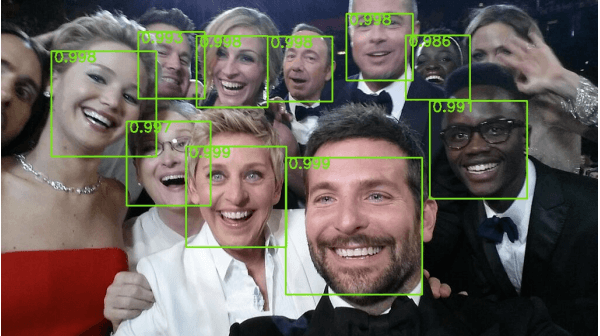
\includegraphics[scale=1]{img/figura-1.png}
\caption{Exemplo de aplicação de Visão Computacional para o reconhecimento de rostos.} 
\label{fig:exemplo-vc}
\end{figure}


Os tópicos seguintes apresentam um panorama: da deficiência físico-motora, Tecnologia Assistiva e o potencial da visão computacional neste meio; a Metodologia utilizado no neste trabalho, descrição e detalhamento do funcionamento do VisiUMouse até a fase de modelagem, Design entre outros.

\begin{comment}
Exemplos do Template
\section{Motivação e objetivos}
\section{Contribuicoes}
\section{Producao cientifica}
\section{Organizacao da tese}
\noindent \textbf{Capitulo \ref{CAP2}}: descricao...
\noindent \textbf{Capitulo \ref{CAP3}}: descricaoo...
\noindent \textbf{Capitulo \ref{CAP4}}: descricao...
\noindent \textbf{Capitulo \ref{CAP5}}: descricao...
\end{comment}